% Generated from the archived contact-error endpoint summary.
% Each point is a mean with sample standard deviation over three repetitions.
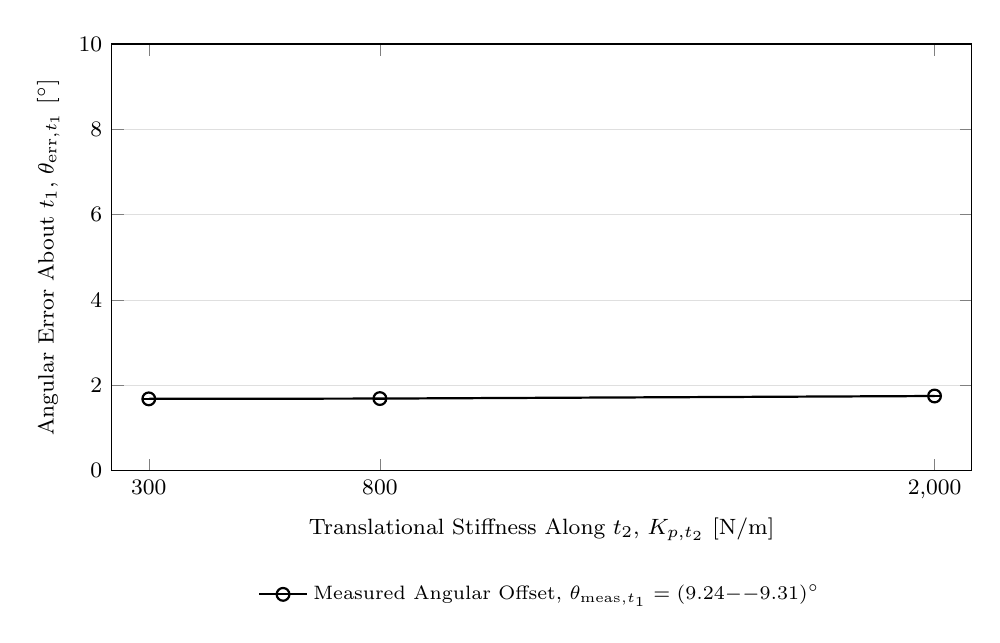
\begin{tikzpicture}
\begin{axis}[
    width=12.5cm, height=7.0cm,
    xmin=220, xmax=2080, ymin=0, ymax=10,
    xtick={300,800,2000}, ytick={0,2,4,6,8,10},
    xlabel={Translational Stiffness Along \(t_2\), \(K_{p,t_2}\) [N/m]},
    ylabel={Angular Error About \(t_1\), \(\theta_{\mathrm{err},t_1}\) [\(^\circ\)]},
    ymajorgrids=true, xmajorgrids=false,
    grid style={gray!25, very thin},
    tick label style={font=\footnotesize},
    label style={font=\footnotesize},
    legend style={font=\scriptsize, draw=none, fill=none,
                  cells={anchor=west}, at={(0.5,-0.24)}, anchor=north},
    every axis plot/.append style={thick, mark size=2.3pt},
  ]
\addplot[black, mark=o, mark options={fill=white},
         error bars/.cd, y dir=both, y explicit] coordinates {
  (300,1.683333333) +- (0,0.011547005)
  (800,1.690000000) +- (0,0.010000000)
  (2000,1.750000000) +- (0,0.000000000)};
\addlegendentry{Measured Angular Offset, \(\theta_{\mathrm{meas},t_1}=(9.24\text{--}9.31)^\circ\)}
\end{axis}
\end{tikzpicture}
